\documentclass[12pt,twoside]{article}
\bibliographystyle{unsrt}

\newcommand{\reporttitle}{Comparing Unsupervised and Supervised Latent Dirichlet Allocation (LDA) for Topic Modeling the STEM Research Funding Landscape in UK}
\newcommand{\reportauthor}{Zitong Zhao}
\newcommand{\reportsupervisor}{Samraat Pawar}
\newcommand{\reporttype}{Coursework}
\newcommand{\cid}{02294840} 

% include files that load packages and define macros
%%%%%%%%%%%%%%%%%%%%%%%%%%%%%%%%%%%%%%%%%
% University Assignment Title Page 
% LaTeX Template
% Version 1.0 (27/12/12)
%
% This template has been downloaded from:
% http://www.LaTeXTemplates.com
%
% Original author:
% WikiBooks (http://en.wikibooks.org/wiki/LaTeX/Title_Creation)
%
% License:
% CC BY-NC-SA 3.0 (http://creativecommons.org/licenses/by-nc-sa/3.0/)
% 
% Instructions for using this template:
% This title page is capable of being compiled as is. This is not useful for 
% including it in another document. To do this, you have two options: 
%
% 1) Copy/paste everything between \begin{document} and \end{document} 
% starting at \begin{titlepage} and paste this into another LaTeX file where you 
% want your title page.
% OR
% 2) Remove everything outside the \begin{titlepage} and \end{titlepage} and 
% move this file to the same directory as the LaTeX file you wish to add it to. 
% Then add \input{./title_page_1.tex} to your LaTeX file where you want your
% title page.
%
%----------------------------------------------------------------------------------------
%	PACKAGES AND OTHER DOCUMENT CONFIGURATIONS
%----------------------------------------------------------------------------------------
\usepackage{ifxetex}
\usepackage{textpos}
\usepackage{natbib}
\usepackage{kpfonts}
\usepackage[a4paper,hmargin=2.8cm,vmargin=2.0cm,includeheadfoot]{geometry}
\usepackage{ifxetex}
\usepackage{stackengine}
\usepackage{tabularx,longtable,multirow,subfigure,caption}%hangcaption
\usepackage{fncylab} %formatting of labels
\usepackage{fancyhdr}
\usepackage{color}
\usepackage[tight,ugly]{units}
\usepackage{url}
\usepackage{float}
\usepackage[english]{babel}
\usepackage{amsmath}
\usepackage{graphicx}
\usepackage[colorinlistoftodos]{todonotes}
\usepackage{dsfont}
\usepackage{epstopdf} % automatically replace .eps with .pdf in graphics
\usepackage{natbib}
\usepackage{backref}
\usepackage{array}
\usepackage{latexsym}
\usepackage{etoolbox}
\usepackage{enumerate} % for numbering with [a)] format 



\ifxetex
\usepackage{fontspec}
\setmainfont[Scale=.8]{OpenDyslexic-Regular}
\else
\usepackage[pdftex,pagebackref,hypertexnames=false,colorlinks]{hyperref} % provide links in pdf
\hypersetup{pdftitle={},
  pdfsubject={}, 
  pdfauthor={\reportauthor},
  pdfkeywords={}, 
  pdfstartview=FitH,
  pdfpagemode={UseOutlines},% None, FullScreen, UseOutlines
  bookmarksnumbered=true, bookmarksopen=true, colorlinks,
    citecolor=black,%
    filecolor=black,%
    linkcolor=black,%
    urlcolor=black}
\usepackage[all]{hypcap}
\fi

\usepackage{tcolorbox}

% various theorems
\usepackage{ntheorem}
\theoremstyle{break}
\newtheorem{lemma}{Lemma}
\newtheorem{theorem}{Theorem}
\newtheorem{remark}{Remark}
\newtheorem{definition}{Definition}
\newtheorem{proof}{Proof}

% example-environment
\newenvironment{example}[1][]
{ 
\vspace{4mm}
\noindent\makebox[\linewidth]{\rule{\hsize}{1.5pt}}
\textbf{Example #1}\\
}
{ 
\noindent\newline\makebox[\linewidth]{\rule{\hsize}{1.0pt}}
}



%\renewcommand{\rmdefault}{pplx} % Palatino
% \renewcommand{\rmdefault}{put} % Utopia

\ifxetex
\else
\renewcommand*{\rmdefault}{bch} % Charter
\renewcommand*{\ttdefault}{cmtt} % Computer Modern Typewriter
%\renewcommand*{\rmdefault}{phv} % Helvetica
%\renewcommand*{\rmdefault}{iwona} % Avant Garde
\fi

\setlength{\parindent}{0em}  % indentation of paragraph

\setlength{\headheight}{14.5pt}
\pagestyle{fancy}
\fancyfoot[ER,OL]{\thepage}%Page no. in the left on
                                %odd pages and on right on even pages
\fancyfoot[OC,EC]{\sffamily }
\renewcommand{\headrulewidth}{0.1pt}
\renewcommand{\footrulewidth}{0.1pt}
\captionsetup{margin=10pt,font=small,labelfont=bf}


%--- chapter heading

\def\@makechapterhead#1{%
  \vspace*{10\p@}%
  {\parindent \z@ \raggedright %\sffamily
        %{\Large \MakeUppercase{\@chapapp} \space \thechapter}
        %\\
        %\hrulefill
        %\par\nobreak
        %\vskip 10\p@
    \interlinepenalty\@M
    \Huge \bfseries 
    \thechapter \space\space #1\par\nobreak
    \vskip 30\p@
  }}

%---chapter heading for \chapter*  
\def\@makeschapterhead#1{%
  \vspace*{10\p@}%
  {\parindent \z@ \raggedright
    \sffamily
    \interlinepenalty\@M
    \Huge \bfseries  
    #1\par\nobreak
    \vskip 30\p@
  }}
  



% %%%%%%%%%%%%% boxit
\def\Beginboxit
   {\par
    \vbox\bgroup
	   \hrule
	   \hbox\bgroup
		  \vrule \kern1.2pt %
		  \vbox\bgroup\kern1.2pt
   }

\def\Endboxit{%
			      \kern1.2pt
		       \egroup
		  \kern1.2pt\vrule
		\egroup
	   \hrule
	 \egroup
   }	

\newenvironment{boxit}{\Beginboxit}{\Endboxit}
\newenvironment{boxit*}{\Beginboxit\hbox to\hsize{}}{\Endboxit}



\allowdisplaybreaks

\makeatletter
\newcounter{elimination@steps}
\newcolumntype{R}[1]{>{\raggedleft\arraybackslash$}p{#1}<{$}}
\def\elimination@num@rights{}
\def\elimination@num@variables{}
\def\elimination@col@width{}
\newenvironment{elimination}[4][0]
{
    \setcounter{elimination@steps}{0}
    \def\elimination@num@rights{#1}
    \def\elimination@num@variables{#2}
    \def\elimination@col@width{#3}
    \renewcommand{\arraystretch}{#4}
    \start@align\@ne\st@rredtrue\m@ne
}
{
    \endalign
    \ignorespacesafterend
}
\newcommand{\eliminationstep}[2]
{
    \ifnum\value{elimination@steps}>0\leadsto\quad\fi
    \left[
        \ifnum\elimination@num@rights>0
            \begin{array}
            {@{}*{\elimination@num@variables}{R{\elimination@col@width}}
            |@{}*{\elimination@num@rights}{R{\elimination@col@width}}}
        \else
            \begin{array}
            {@{}*{\elimination@num@variables}{R{\elimination@col@width}}}
        \fi
            #1
        \end{array}
    \right]
    & 
    \begin{array}{l}
        #2
    \end{array}
    &%                                    moved second & here
    \addtocounter{elimination@steps}{1}
}
\makeatother

%% Fast macro for column vectors
\makeatletter  
\def\colvec#1{\expandafter\colvec@i#1,,,,,,,,,\@nil}
\def\colvec@i#1,#2,#3,#4,#5,#6,#7,#8,#9\@nil{% 
  \ifx$#2$ \begin{bmatrix}#1\end{bmatrix} \else
    \ifx$#3$ \begin{bmatrix}#1\\#2\end{bmatrix} \else
      \ifx$#4$ \begin{bmatrix}#1\\#2\\#3\end{bmatrix}\else
        \ifx$#5$ \begin{bmatrix}#1\\#2\\#3\\#4\end{bmatrix}\else
          \ifx$#6$ \begin{bmatrix}#1\\#2\\#3\\#4\\#5\end{bmatrix}\else
            \ifx$#7$ \begin{bmatrix}#1\\#2\\#3\\#4\\#5\\#6\end{bmatrix}\else
              \ifx$#8$ \begin{bmatrix}#1\\#2\\#3\\#4\\#5\\#6\\#7\end{bmatrix}\else
                 \PackageError{Column Vector}{The vector you tried to write is too big, use bmatrix instead}{Try using the bmatrix environment}
              \fi
            \fi
          \fi
        \fi
      \fi
    \fi
  \fi 
}  
\makeatother

\robustify{\colvec}

%%% Local Variables: 
%%% mode: latex
%%% TeX-master: "notes"
%%% End: 
 % various packages needed for maths etc.
% quick way of adding a figure
\newcommand{\fig}[3]{
 \begin{center}
 \scalebox{#3}{\includegraphics[#2]{#1}}
 \end{center}
}

%\newcommand*{\point}[1]{\vec{\mkern0mu#1}}
\newcommand{\ci}[0]{\perp\!\!\!\!\!\perp} % conditional independence
\newcommand{\point}[1]{{#1}} % points 
\renewcommand{\vec}[1]{{\boldsymbol{{#1}}}} % vector
\newcommand{\mat}[1]{{\boldsymbol{{#1}}}} % matrix
\newcommand{\R}[0]{\mathds{R}} % real numbers
\newcommand{\Z}[0]{\mathds{Z}} % integers
\newcommand{\N}[0]{\mathds{N}} % natural numbers
\newcommand{\nat}[0]{\mathds{N}} % natural numbers
\newcommand{\Q}[0]{\mathds{Q}} % rational numbers
\ifxetex
\newcommand{\C}[0]{\mathds{C}} % complex numbers
\else
\newcommand{\C}[0]{\mathds{C}} % complex numbers
\fi
\newcommand{\tr}[0]{\text{tr}} % trace
\renewcommand{\d}[0]{\mathrm{d}} % total derivative
\newcommand{\inv}{^{-1}} % inverse
\newcommand{\id}{\mathrm{id}} % identity mapping
\renewcommand{\dim}{\mathrm{dim}} % dimension
\newcommand{\rank}[0]{\mathrm{rk}} % rank
\newcommand{\determ}[1]{\mathrm{det}(#1)} % determinant
\newcommand{\scp}[2]{\langle #1 , #2 \rangle}
\newcommand{\kernel}[0]{\mathrm{ker}} % kernel/nullspace
\newcommand{\img}[0]{\mathrm{Im}} % image
\newcommand{\idx}[1]{{(#1)}}
\DeclareMathOperator*{\diag}{diag}
\newcommand{\E}{\mathds{E}} % expectation
\newcommand{\var}{\mathds{V}} % variance
\newcommand{\gauss}[2]{\mathcal{N}\big(#1,\,#2\big)} % gaussian distribution N(.,.)
\newcommand{\gaussx}[3]{\mathcal{N}\big(#1\,|\,#2,\,#3\big)} % gaussian distribution N(.|.,.)
\newcommand{\gaussBig}[2]{\mathcal{N}\left(#1,\,#2\right)} % see above, but with brackets that adjust to the height of the arguments
\newcommand{\gaussxBig}[3]{\mathcal{N}\left(#1\,|\,#2,\,#3\right)} % see above, but with brackets that adjust to the height of the arguments
\DeclareMathOperator{\cov}{Cov} % covariance (matrix) 
\ifxetex
\renewcommand{\T}[0]{^\top} % transpose
\else
\newcommand{\T}[0]{^\top}
\fi
% matrix determinant
\newcommand{\matdet}[1]{
\left|
\begin{matrix}
#1
\end{matrix}
\right|
}



%%% various color definitions
\definecolor{darkgreen}{rgb}{0,0.6,0}

\newcommand{\blue}[1]{{\color{blue}#1}}
\newcommand{\red}[1]{{\color{red}#1}}
\newcommand{\green}[1]{{\color{darkgreen}#1}}
\newcommand{\orange}[1]{{\color{orange}#1}}
\newcommand{\magenta}[1]{{\color{magenta}#1}}
\newcommand{\cyan}[1]{{\color{cyan}#1}}


% redefine emph
\renewcommand{\emph}[1]{\blue{\bf{#1}}}

% place a colored box around a character
\gdef\colchar#1#2{%
  \tikz[baseline]{%
  \node[anchor=base,inner sep=2pt,outer sep=0pt,fill = #2!20] {#1};
    }%
}%
 % short-hand notation and macros


%%%%%%%%%%%%%%%%%%%%%%%%%%%%
\begin{document}
% front page
% Last modification: 2016-09-29 (Marc Deisenroth)
\begin{titlepage}

\newcommand{\HRule}{\rule{\linewidth}{0.5mm}} % Defines a new command for the horizontal lines, change thickness here


%----------------------------------------------------------------------------------------
%	LOGO SECTION
%----------------------------------------------------------------------------------------


\includegraphics[width = 4cm]{./figures/imperial}\\[0.5cm] 

\begin{center} % Center remainder of the page

%----------------------------------------------------------------------------------------
%	HEADING SECTIONS
%----------------------------------------------------------------------------------------
\textsc{\LARGE \reporttype}\\[1.5cm] 
\textsc{\Large Imperial College London}\\[0.5cm] 
\textsc{\large Department of Computing}\\[0.5cm] 
%----------------------------------------------------------------------------------------
%	TITLE SECTION
%----------------------------------------------------------------------------------------

\HRule \\[0.4cm]
{ \huge \bfseries \reporttitle}\\ % Title of your document
\HRule \\[1.5cm]
\end{center}
%----------------------------------------------------------------------------------------
%	AUTHOR SECTION
%----------------------------------------------------------------------------------------

%\begin{minipage}{0.4\hsize}
\begin{flushleft} \large
\textit{Author:}
\reportauthor~(CID: \cid) % Your name
\\
\textit{Supervisor:}
\reportsupervisor~
\end{flushleft}
\vspace{2cm}
\makeatletter
Date: \@date \\
Word Count: 5992
\vfill % Fill the rest of the page with whitespace
\begin{center}
\textbf{A thesis submitted in partial fulfilment of the requirements for the degree of Master of Science at Imperial College London}\\
\textbf{Submitted for the MSc in Computational Methods in Ecology and Evolution}
\end{center}

\makeatother


\end{titlepage}


\newpage
\thispagestyle{empty} 

\section*{Declaration}
I declare The data used in this dissertation was provided by Bellotto Trigo, Flavia and Pawar, Samraat. \\\\
I declare that I am responsible for the processing visualisation and analysis of the data. \\\\
I would like to extend special gratitude to my supervisor Samraat Pawar, for his dedicated guidance and assistance throughout the research process.
\\\\


\tableofcontents

\newpage
\begin{abstract}
Topic modeling is one of the most powerful techniques in text mining, utilized for data mining, latent data discovery, and identifying relationships between data and text documents. Latent Dirichlet Allocation (LDA) is one of the most popular methods in this field. Additionally,I will introduce a supervised variant of LDA called supervised Latent Dirichlet Allocation (sLDA), which leverages labelled data to classify document topics. The model results for sLda contain estimated parameters, which are used to describe the relationship between labels and topic. The comparison and evaluation of unsupervised and supervised LDA models involve metrics such as semantic coherence, complexity, and visualisations of high-probability words per topic, providing deeper insights. Through the comparison of LDA and sLDA models, this study enhances people understanding of topic modeling in text analysis applications. The dataset used is the research funding information from the UK Research and Innovation (UKRI). By analyzing the distribution of funding within UKRI, it is possible to gain insights into the disciplines at the forefront of development, facilitate interdisciplinary research, and optimize the allocation of funds.

\end{abstract}
\section{Introduction}
In today's era of vast electronic text collections, there is an increasing demand for analysing and understanding such large datasets. Natural Language Processing (NLP) is a challenging field of study in computer science that involves information management, semantic mining, and enabling computers to extract meaning from human language processing within text documents \cite{Jelodar:2019aa}. Topic modeling methods are powerful technologies widely applied in natural language processing, enabling the discovery of themes in unstructured documents and semantic mining \cite{blei2003latent} and has a wide range of applications in various fields \cite{Varghese:2018aa} \cite{Papadatos:2014aa}.\\\\

The project focuses on comparing the practicality of unsupervised learning and supervised learning in natural language processing. The dataset used is the research funding information from the UK Research and Innovation (UKRI), and topic modeling is employed to classify the distribution of STEM (Science, Technology, Engineering, and Mathematics) disciplines. Subsequently, an analysis is conducted based on the classification results. UKRI is a government-established organization with the aim of advancing the UK's position as a global leader in science, technology, and socio-economic development. It achieves this by providing support and funding for various activities, including research, innovation, and higher education. This organization contains numerous approved research proposals, and in this article, we will employ natural language processing to conduct topic analysis and categorize all these proposals. Analyzing the distribution of UKRI funding allows us to gain insights into the research directions and significance of various STEM disciplines. It provides valuable information on which disciplines are at the forefront of development. This, in turn, can promote collaboration and communication between different disciplines, foster interdisciplinary research, and optimize the allocation of funding, ensuring a fair distribution and maximizing its impact.\\\\

To classify a large number of unordered documents into topics, one powerful approach for this task is the Latent Dirichlet Allocation (LDA) model which introduced by Blei et al. were utilized as a novel approach for document classification (\cite{blei2003latent}, \cite{blei2012probabilistic}), allows us to uncover the underlying themes or topics within documents and the distribution of words within those topics. Interest in incorporating prior information into the topic modeling process has grown, with several effective methods developed to model various types of prior information, such as observed labels, latent labels, inter-label correlations, and label frequencies \cite{Wang:2020aa}. Additionally, a supervised parameter estimation method based on category and document information can estimate the parameters of LDA according to term weight, while to infer the latent topics that predict the responses, a supervised topic model was developed \cite{Liu2015}. One of the advantages of supervised LDA compared to unsupervised LDA is that it can learn topics that align with class labels \cite{Lakshminarayanan2011}. Therefore, extending LDA to supervised algorithms is a hot research topic. supervised-LDA is a type of topic model in supervised learning that constrains LDA by defining a one-to-one correspondence between the latent topics of LDA and user labels (\cite{ramage2009labeled}). Supervised-LDA can directly learn the correspondence between topics and labels. There are also other methods, such as deep learning approaches like CNN, that can be employed for sentiment analysis in topic modeling \cite{Mohammed:2019aa} \cite{Ombabi:2020aa}.\\\\

In this study, I propose to use a supervised LDA model that leverages label information to guide the learning process of the topic model, leading to a more accurate correspondence between topics and labels. As a result, we expect the labeled LDA model to outperform traditional unsupervised LDA models in classification tasks. Through this research, I aim to validate the utility of machine learning in topic classification and demonstrate the potential of supervised LDA in achieving improved performance in classifying research proposals, providing valuable insights into the landscape of research across various STEM disciplines funded by UKRI.


\section{Methodology}

\subsection{Text Data and Label Preprocessing}

The dataset used is the research funding information from the UK Research and Innovation (UKRI). After obtaining a dataset of 85,000 UKRI-funded projects, I initiated the necessary preprocessing steps. This encompassed data cleansing, removing irrelevant characters, special symbols, and non-textual content. Subsequently, I segmented each text into distinct words or tokens, ensuring the text's analyzability. Following this, I converted all words to lowercase to address potential issues of word repetition due to varying cases. After removing common stop words, I performed either stemming or lemmatization on the words, transforming them into their base forms. Eventually, I transformed the tokenized text into a document-term matrix, where each row represents a document, and each column represents a word, thus laying the foundation for subsequent analyses \cite{kochmar2022getting}. \\\\

Each project file contains information about its funding institution, project start and end dates, as well as the total funding amount. I will process this information to derive the labels that I will use for sLDA analysis. Specifically, I will extract the funding institution, funding amount, ubsequently compute the project's duration and the annual funding amount. These processed values will then be used as labels for the sLDA analysis. A major limitation of supervised learning methods is that they assume the provided labels cover all the classes \cite{Kang2014}. \\\\

After document preprocessing, we trimmed documents with fewer than 20 words and removed documents with missing labels, resulting in a final set of 72,686 documents with clean data. After obtaining the cleaned data, I proceed by splitting 75\% of the documents as the training set for our utilisation. Initially, I create a corpus from the text data of the training set and then transform this corpus into tokens, essentially dividing the text into individual linguistic units. Subsequently, these tokens are converted into a document-term matrix (DTM). Following this process, we proceed to employ this document-term matrix for subsequent model fitting and evaluation assessment.

\subsection{Description of the Utilized Model and Analysis Approach}
The LDA model operates by using Markov Chain Monte Carlo (MCMC) method for assigning each word in a document to a specific topic based on the topic distribution of that document. By using a fitted LDA model, we can infer the topic structure of an document and make predictions based on this structure. Our goal is to determine the potential topic probability distribution for each document and the potential word probability distribution for each topic. Subsequently, we aim to infer the topics that maximize the posterior probability.

LDA makes two key assumptions:
\begin{itemize}
\item Documents are referred to as probability densities (or distributions) of topics. Each document is a composition of multiple topics, Each topic is associated with a probability. For instance, Document 1 is composed of 65\% of Topic 1, 10\% of Topic 2, and so on. This signifies that a document might encompass multiple topics simultaneously, with certain topics being more relevant due to higher probabilities. 

\item Topics are probability densities (or distributions) of words. Each topic is comprised of a distribution of words. For example, Topic 1 consists of 77\% of Word 1, 12\% of Word 2, and so forth. 
\end{itemize}
The relationship of probabilities between documents, topics, and words underpins the model \cite{Seth2021}.\\\\

Probability distributions in the LDA model can be summarised as the Dirichlet distribution acts as a prior. It influences the topic distribution in each document and the word distribution in each topic during document generation. Likelihood refers to the probability of generating a document based on known topic and word distributions. The posterior distribution calculates the probability of topic and word distributions given documents and model parameters \cite{Naushan2020}. 

During the construction of the LDA model, Gibbs sampling is used, which is a specific instance of the MCMC method for sampling from complex multidimensional probability distributions and generating topic distributions and word assignments. Its fundamental concept involves iteratively sampling variables one by one, given the values of other variables, thereby progressively approximating the desired joint distribution. The model-based classification approach of Supervised-LDA requires slightly more additional computation during the testing phase compared to LDA\cite{Lakshminarayanan2011}.

In the initialisation process, a random topic is assigned to each word within each document. According to LDA, each word is linked to a latent (or hidden) topic. During the iteration, the probability for a word $w$ to belong to a topic $t$ is calculated the product of this two factors: $p(\text{topic } t \mid \text{document } d)$ and $p(\text{word } w \mid \text{topic } t)$ \cite{Kulshrestha2019}.The former represents the proportion of words assigned to topic $t$ within document $d$, demonstrating the relevance between topic $t$ and the content of document $d$. The latter signifies the proportion of assignments to topic $t$ from word $w$ across all documents, illustrating the association of word $w$ with topic $t$ across the entire corpus. Based on this conditional probability distribution, a new topic is drawn from the possible topics to update the topic assignment for the current word. After a certain number of iterations, the model converges and attains a stable distribution of topics. Each word within each document is ultimately assigned a definitive topic. LDA endeavors to identify an appropriate distribution of topics and word assignments, maximizing the model's ability to generate documents effectively.\\\\

In this study, we employ a comprehensive evaluation approach to assess the performance of topic models, incorporating both qualitative and quantitative metrics. For quantitative evaluation, we utilize two widely-used metrics: coherence and perplexity. Coherence assesses semantic consistency within topics, while perplexity measures the model's predictive performance on unseen data. Regarding qualitative evaluation, I employed both human judgment and observation-based assessment. Based on my analysis of the subject categories of UKRI-funded projects, I conducted an evaluation based on the top 20 words of each topic to generate thematic summaries. This approach allowed for a comprehensive qualitative assessment of the topics and their alignment with the subject matter of the projects.\\\\

By combining qualitative and quantitative evaluation methods, this study offers a comprehensive analysis of topic models' performance and usefulness in text analysis applications. I will visualize the results by highlighting the words with the highest probability of belonging to each topic, providing further insights into the identified topics.

\subsection{Programming Language and Tools Utilized}

I utilized the R programming language to implement LDA and sLDA model. For LDA I used the 'topicmodels' package, which was developed by David M. Blei. LDA operates by probabilistically assigning each word in a document to a specific topic based on the topic distribution of that document.I utilized the 'slda' package to implement sLDA model, which was developed by Matthew J. Denny, to implement sLDA. Unlike traditional LDA, sLDA allows us to incorporate prior knowledge from labeled data to enhance the accuracy of topic classification. The slda package provides functionalities for fitting sLDA models and estimating parameters that describe the relationship between labels and topics. I employed the 'text2vec' package, developed by S. Dmitriy. This package offers a range of tools to calculate coherence for topic models, aiding in the assessment of topic quality. It implements various metrics to evaluate topics represented as ordered term lists. 




\subsection{Coherence}

When dealing with a vast dataset of more than 70 thousands UKRI projects, selecting the right number of topics is critical for effective topic modeling. I chose a range of 50 to 500 topics. The dataset covers STEM disciplines and is diverse. Expanding the topic range to 500 captures this diversity well and prevents losing valuable insights due to fewer topics. However, excessive topic numbers can result in redundancy and complexity. After analyzing the UKRI disciplines, I've set the upper limit at 500. The chosen topic range balances dataset complexity and model interpretability, leading to accurate and insightful results.\\\\

After obtaining the topic classification data generated by both the LDA and sLDA models, I will proceed to assess the coherence of the topics. Topic Coherence measures score a single topic by measuring the degree of semantic similarity between high probability words in the topic \cite{Kapadia2019}. When evaluating coherence, several metrics are employed to assess the consistency of topics by machine learning(\cite{Selivanov2016}), including logarithmic ratio (Eq. 1), pointwise mutual information (Eq. 2), difference (Eq. 3), and Cosim (cosine of normalized PMI). These indicators help determine the level of coherence by analyzing the relationships between individual top words and other top words within a topic. All four of these metrics indicate that larger values correspond to better semantic coherence of the model.

\begin{equation}
    \text{logratio} = \log(\varepsilon + T[x,y]) - \log(T[y,y])
\end{equation}

\begin{equation}
    \text{PMI} = \log_2\left(\frac{T[x,y]}{n_{\text{doc}}} + \varepsilon\right) - \log_2\left(\frac{T[x,x]}{n_{\text{doc}}}\right) - \log_2\left(\frac{T[y,y]}{n_{\text{doc}}}\right)
\end{equation}

\begin{equation}
    \text{Difference} = \frac{T[x,y]}{T[x,x]} - \left(\frac{T[y,y]}{n_{\text{windows}}}\right)
\end{equation}

In those equations, \(\varepsilon\) is the smoothing factor. \(T\) is the term co-occurrence matrix (which objective is to capture the co-occurrence relationships among words within a text, representing the frequency with which words appear in the same context), and \(T[x,y]\) typically refers to the co-occurrence count or frequency of the word "x" and the word "y" within a given set of documents, indicating a potential semantic relationship or thematic connection between them.\(T[y,y]\) represents the total number of documents used in the calculation of the term co-occurrence matrix. \(n_{\text{windows}}\) refers to the total number of context windows used for generating the term co-occurrence matrix. A context window is a specified range of tokens surrounding a target token within a text or sequence. In evaluating the coherence of topics by examining the values of these four coherence measurement metrics, The larger the coherence metrics for topics, the more pronounced the overall model's advantage becomes. Higher coherence scores indicate that within specific topics, there is a tighter semantic correlation between words, resulting in stronger mutual coherence among them. Consequently, such a scenario often signifies that the topic model is better able to accurately capture and express the underlying semantic structure hidden within the text data. When assessing the effectiveness and performance of topic models, comparing coherence scores across different topics allows us to draw a more comprehensive and reliable assessment of the overall model's quality.\\\\

When evaluating topic models, human judgment through topic consistency evaluation is a common approach. This method involves manually reading and analyzing each generated topic from the model to assess its consistency and interpretability.

\subsection{Perplexity}

To decide on a suitable number of topics, Perplexity-K curve is utilized to decide the optimal K-value \cite{Huang2017}. Perplexity is a widely used metric in topic modeling to evaluate the predictive performance of models. It measures how well a model predicts a new set of data given the learned topic distributions. In our study, perplexity was calculated for both the LDA and sLDA models. The perplexity values were obtained by computing the exponential of the negative log-likelihoods of the respective models on the test dataset (\cite{wallach2009evaluation}).

\begin{equation}
        \text{Perplexity} = \exp \left\{ -\frac{{\sum_{d=1}^{M} \log p(\mathbf{w}_d)}}{{\sum_{d=1}^{M} N_d}} \right\}
\end{equation}


\(M\) is the number of documents, \(\mathbf{w}_d\) represents the words in document \(d\), \(N_d\) the total number of words in document \(d\). \(p(\mathbf{w}_d)\) is the likelihood of document 
\(d\), which is calculated from the model's learned topic distributions.\\\\

Perplexity provides an effective way to measure how well these models can predict unseen data based on the learned topic distributions. A lower perplexity value indicates better predictive performance and suggests that the model's topic assignments align well with the actual test data.



\section{Results}
\subsection{Exploring Topics and Insights from the LDA Model}
In this section, I present a comparative analysis between Latent Dirichlet Allocation (LDA) and Supervised Latent Dirichlet Allocation (sLDA), focusing on their respective performances and capabilities. Both LDA and sLDA are powerful probabilistic topic modeling techniques used for extracting latent structures from text data. Our goal is to highlight the key differences and advantages of these two approaches in various aspects.\\\\


In Figure 1, I visualized the topic-word probability matrix of the LDA model which is the posterior distribution of words and documents to topics, and randomly selected a few intuitive topics to examine the generated results, it shows topics are probability distributions of words. Additionally, the word clouds visually represent terms in proportions corresponding to their frequency of occurrence \cite{vanAtteveldt2018}. In each topic's word cloud, it can be observed that the included words exhibit a certain level of correlation. This indicates the capability of the LDA model to categorize text by grouping words with similar semantics. Such clustering aids in identifying commonalities between topics, forming distinctive features, and extracting latent themes from the text.\\\\

The size of words indicates their equal probabilities within that specific topic.For example, in Figure 1 (a), these probabilities can infer that this topic is associated with concepts such as females, pregnancy, babies, childbirth, risk, and mothers. This aids in understanding the model's ability to capture and express latent topics within the data.\\\\

\begin{figure}[htbp]
    \centering
    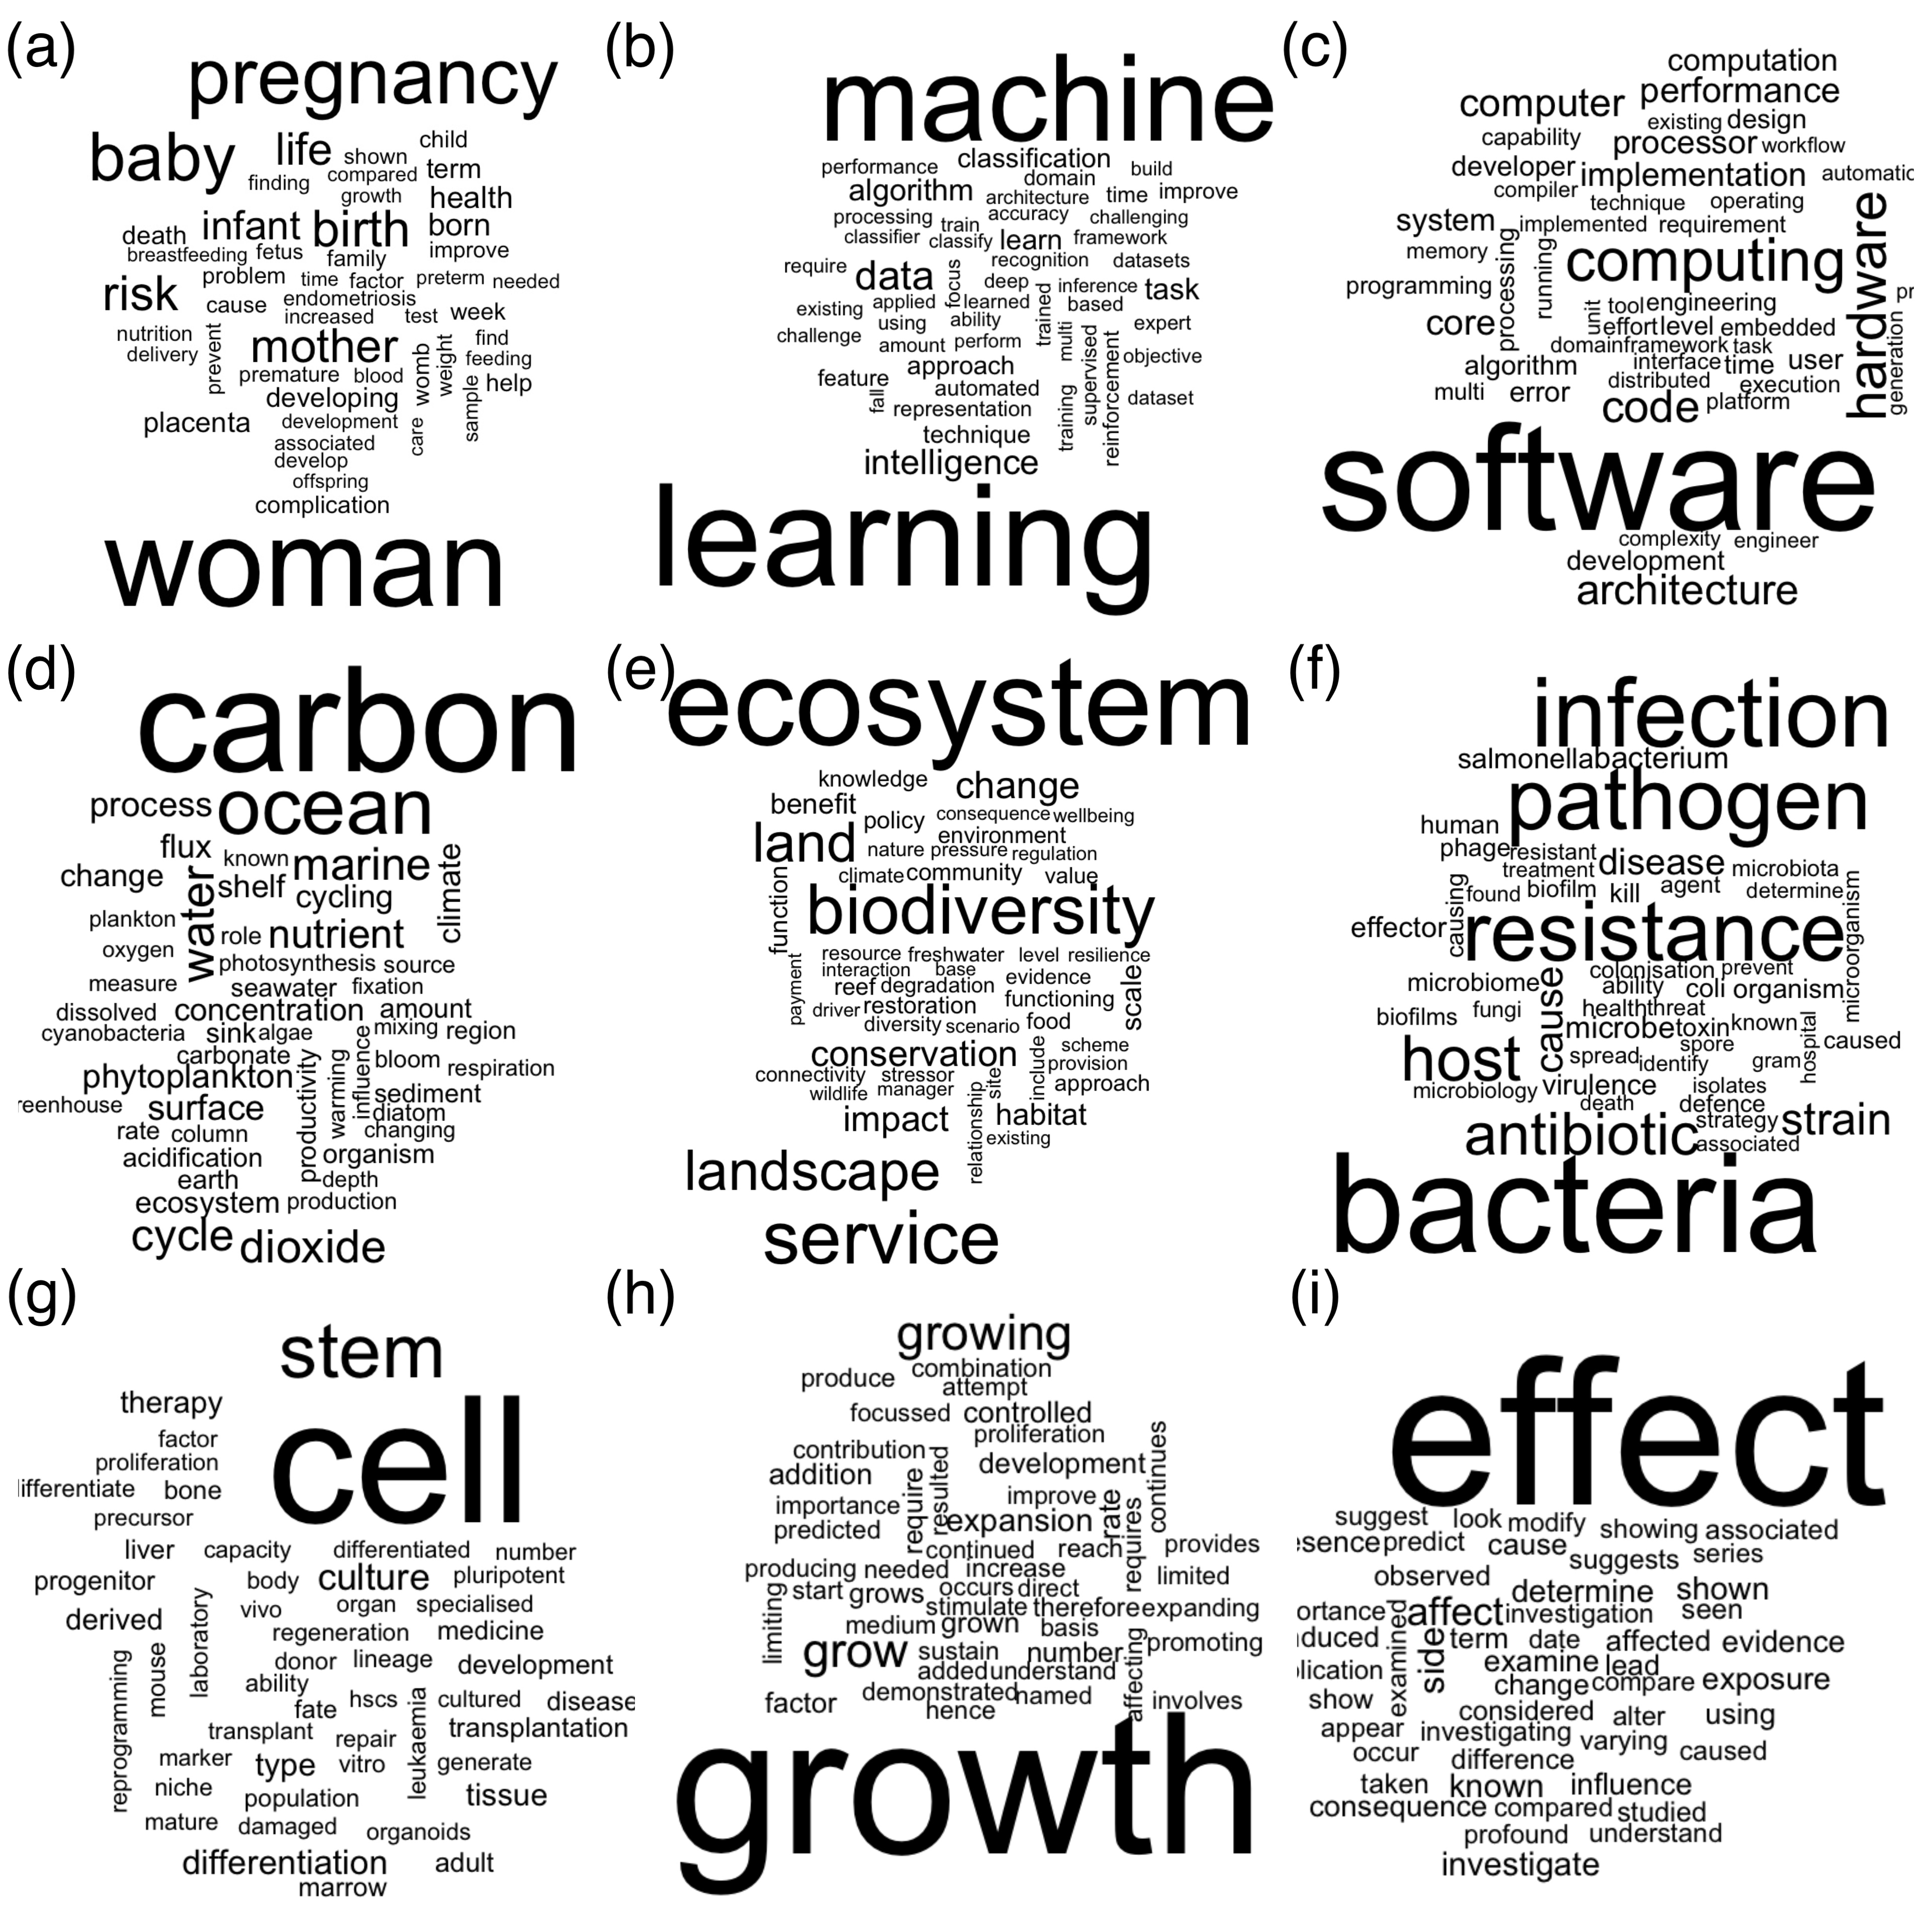
\includegraphics[width=14cm]{./figures/IMG_5754}\\[0.15cm] 
    \caption{The topic-word probability matrix visualisation of 225-topics LDA model by 'Wordcloud'. These are the topics number 31, 64, 179, 184, 39, 93, 81, 166, and 204 that I selected by their words. The size of words indicates their probabilities within that specific topic.}

\end{figure}

In Figure 1 (d, e), both visualisations pertain to the field of environmental science. The common keyword in both visualisations is 'ecosystem.' In visualisation (e), the term 'ecosystem' holds significant prominence across the entire topic, signifying its central importance. In contrast, in Figure 1 (d), the term 'ecosystem' (shown at the bottom) holds a relatively lower probability within the topic. This suggests that the word might possess polysemy or different semantic associations in distinct contexts. This underscores a characteristic of topic models like LDA – they can reveal the complexity of word polysemy and semantic associations across various contexts. This aspect is crucial for extracting deeper insights and meanings from text data.\\\\

In Figures (h, i), we observe topics mainly as 'growth' and 'effect'. However, these words possess rather general meanings. Consequently, we face difficulty in precisely determining the subject matter of these topics. This uncertainty arises because these words can be applicable in various contexts, such as economy or data-related discussions, potentially relating to the concepts of growth and effect.\\\\


This highlights the capabilities of the LDA model in aiding our understanding of inter-topic relationships, identifying commonalities, uncovering latent topics, and addressing the complexities of word polysemy and semantic associations. These insights hold significant value in the realms of text analysis, topic mining, and information extraction.

\subsection{Enhanced Term Coherence by Increased Term Co-occurrence Frequency Difference in sLDA through Label Information}

The coherence measures the semantic similarity among words within a topic. It evaluates the inherent connections between words within a specific topic context, reflecting the meanings and conceptual associations of these words within that topic. When studying topics within UKRI projects, we explore the degree of correlation across different domains such as environmental science and healthcare, aiming to enhance our understanding of word similarity within topics.\\\\

In the context of comparing LDA and SLDA models, the computation of topic coherence becomes particularly crucial. By comparing the topic coherence scores generated by both models, it reveals which model excels in accurately capturing the semantic relationships between words. This process aids in deepening our comprehension of how well the models perform in uncovering hidden topics within the textual data of UKRI projects.\\\\


\begin{figure}[h]
    \centering
    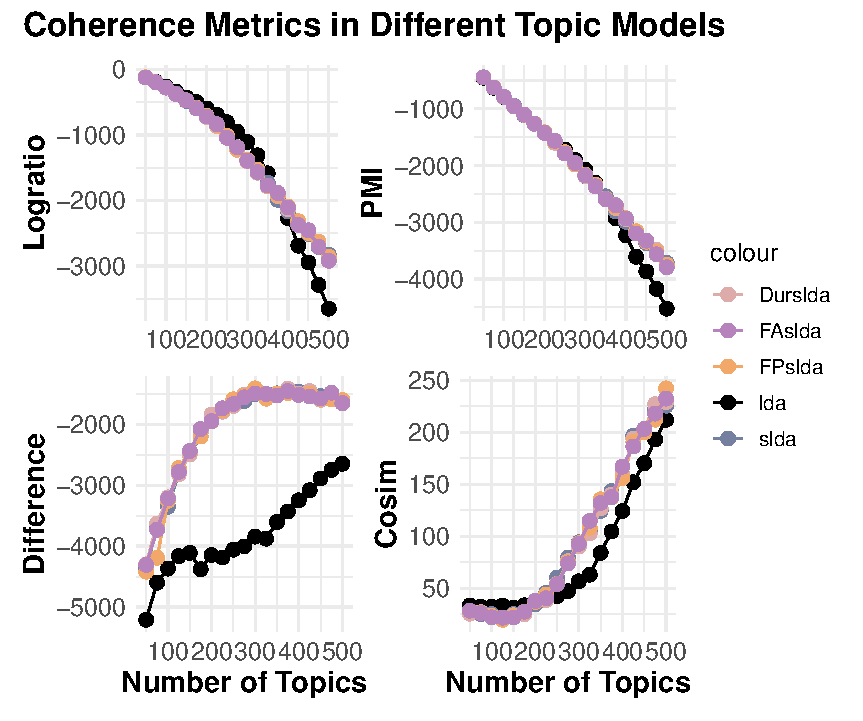
\includegraphics[width=15cm]{./figures/Coherence}\\[0.2cm] 
    \caption{Four coherence measurement metrics across topics ranging from 50 to 500 for both LDA and sLDA models}

\end{figure}

Figure 2 displays the results of four coherence measurement metrics across topics ranging from 50 to 500 for both LDA and sLDA models. The calculation involves the frequency between two terms within the top 20 terms of the topic-word probability matrix of both the LDA and sLDA models. Compared to other metrics, 'difference' places greater emphasis on the distinctiveness between different terms, highlighting both the frequency disparities among terms and their prominence within specific contexts. Therefore, a larger frequency difference is generally considered more favorable for the model.\\\\

In terms of 'logratio' and 'pmi' metrics, both LDA and sLDA exhibit similar performances. At smaller numbers of topics, LDA might excel in capturing textual coherence and co-occurrence relationships, thus demonstrating better performance in the early stages. However, as the number of topics increases, sLDA might better adapt to more intricate semantic relationships and inter-topic interactions, resulting in improved performance with larger topic counts. This transition potentially reflects the underlying strengths and adaptability of LDA and sLDA across varying scales of topics.\\\\

In terms of the 'difference' and 'cosim' metrics, sLDA tends to outperform LDA, which suggests that sLDA holds an advantage in capturing the frequency differences and semantic similarities between terms. Additionally, sLDA exhibits greater proficiency in handling diversity, semantic associations, and topic interactions. By considering label information, sLDA might compute term frequency differences more accurately, leading to higher values when measuring term distinctiveness in the difference metric. Furthermore, the sLDA model introduces label information on top of the LDA foundation, enhancing the semantic representation of terms and enabling the model to establish stronger connections between terms and labels.


\subsection{Determine Optimal Topic Counts and Evaluate the LDA and sLDA Models Using Perplexity}

To make a robust comparison between the LDA and sLDA models and assess the goodness-of-fit and the best topic counts, perplexity calculation serves as a crucial evaluation criterion. Additionally, we sought to identify the optimal number of topics for each model, which further highlights the importance of perplexity analysis in our study.\\\\

To calculate perplexity for both models, we utilized the log-likelihood values obtained during model training and then transformed them using the exponential function. The resulting perplexity values provide a quantitative measure of how well the models generalize to new data.\\\\

\begin{figure}[h]
    \centering
    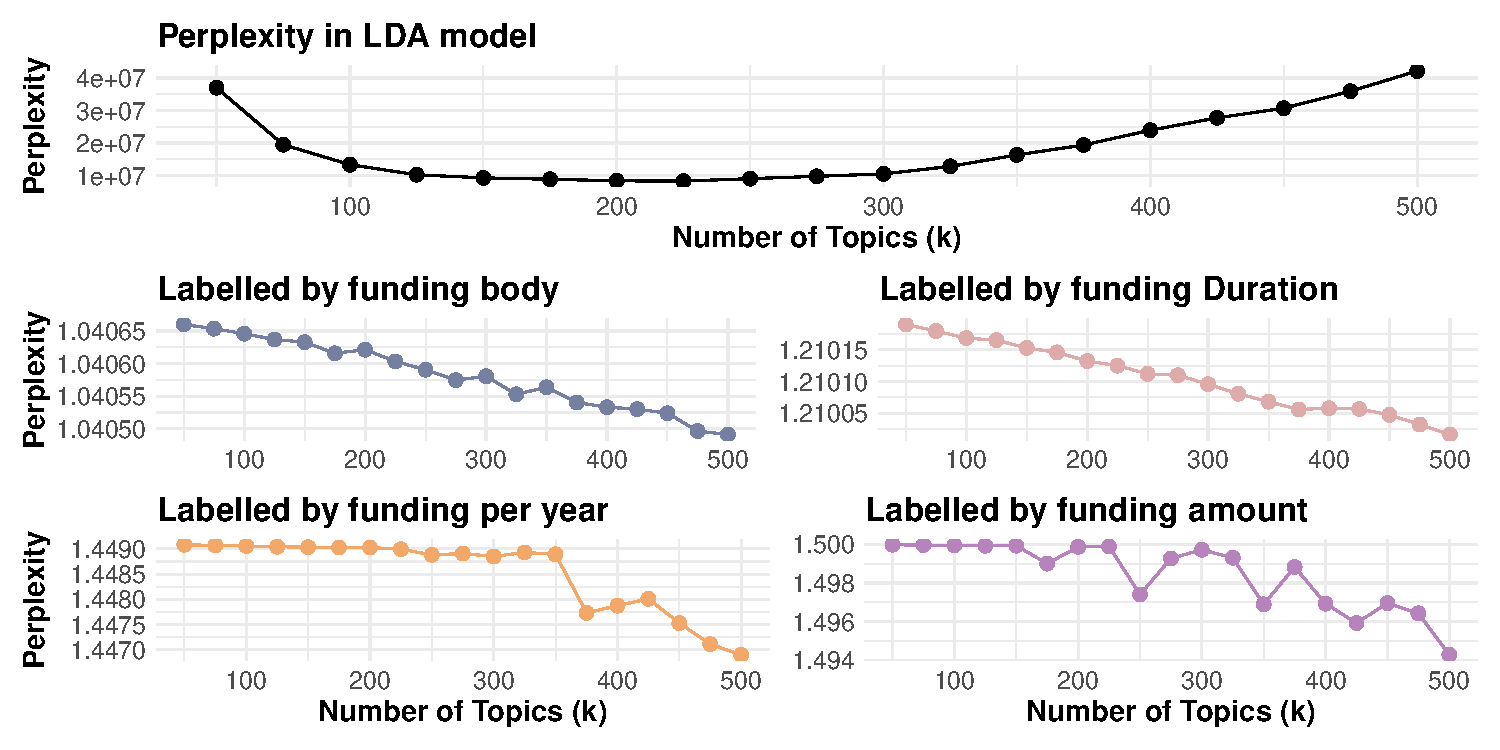
\includegraphics[width=15cm]{./figures/lda-slda}\\[0.2cm] 
    \caption{This is the perplexity of the lda model and the slda model in different topics. The slda models have different labels.}

\end{figure}


The perplexity of the LDA model reached around 2e+07 (in Fig.3), while the perplexity of various labeled sLDA models ranged from 1 to 1.4. This difference could be attributed to the fact that the sLDA model, after incorporating label information, effectively leveraged the underlying structure and latent patterns in the data, leading to superior performance in prediction and lower perplexity.\\\\

The LDA model may experience an increase in perplexity due to it overly fit the existing training data, resulting in poorer performance on unseen new text data. Elevated perplexity implies that the model struggles to predict new text data, making it challenging to accurately discern the topics or categories to which the text belongs. Therefore, even though the LDA model might exhibit impressive performance on the training data, its predictive ability could be compromised by its complexity, leading to poorer performance on new text data.\\\\

In the lda model, perplexity is lowest when the number of topics is around 225. This suggests that, on this specific dataset, the LDA model exhibits relatively optimal predictive ability when using approximately 225 topics. Above 225 topics, the perplexity starts to get gradually larger. In traditional LDA models, an increase in the number of topics may lead to overfitting or a rise in model complexity, so that at some point the perplexity starts to rise, creating a clear nadir.\\\\

However, it can be seen that in slda, perplexity is generally and consistently decreasing as the number of topics increases. The reason is that with a larger number of topics, the sLDA model can become increasingly flexible and better equipped to adapt to complex data distributions and text structures. It can further partition each topic into more specific subcategories, thereby enhancing its ability to represent the text data. This finer-grained classification allows the model to more accurately capture subtle differences between data points, resulting in a gradual reduction of perplexity. Furthermore, the sLDA model with an increasing number of topics might be more effective in classifying texts based on the provided label information. This capability enables the model to more accurately identify differences between various topics, resulting in a gradual decrease in perplexity as the number of topics grows.\\\\

After calculating and comparing the perplexity values of the LDA and sLDA models, we found that the sLDA model performs superior in fitting the data. sLDA demonstrates significant performance in prediction, hence possessing superior predictive and categorization capabilities when dealing with new text data. This results in a notable improvement in perplexity during corresponding evaluations. It can also be stated that the LDA model yields satisfactory outcomes in the analysis of the current dataset; however, its classification performance is evidently less impressive when confronted with entirely new text data.

\subsection{Parameter Estimation for Supervised LDA Using Category and Document Information}
The sLDA model is additionally capable of estimating the labels associated with each topic it classifies, thereby allowing for parameter estimation in sLDA based on term weights. After training the sLDA model using the slda.em algorithm in R, the results can be accessed to examine the associations between each topic and corresponding labels. Typically,
the output of sLDA model includes Estimate value. This estimates of the sLDA model are obtained through the optimization of the joint probability of text data and label information. During the training process, the model searches for the optimal parameter settings to maximize the likelihood of the data and determine the probability relationship between each topic and its associated label. These estimated values help us understand the structure and patterns within the text data, providing valuable information for tasks such as text classification, topic analysis, and other natural language processing tasks.\\\\


Figure 4 visually presents an analysis outcome of the SLDA model through data visualisation. I chose a topic number of 75 for a complete presentation and analysis. In the case of a smaller number of topics, we found that the estimated values of sLDA were quite close in this example. The data reveals a distinct pattern where the estimates are predominantly clustered within the range of 800 to 1000. This specific trend is related to the 'technology' topic, indicating that projects classified under the 'technology' category exhibit relatively shorter projected duration. The proximity of sLDA's estimated values could be attributed to the relatively lower complexity of the model under fewer topics, making it more likely to converge to similar estimation results. When the number of topics is relatively low, such as 75, the model's expressive capability is relatively weak, potentially leading to an insufficient capture of the data's complexity and subtle differences. As a result, the estimates tend to cluster around a narrower range, which is between 800 and 1000 in this case. With a smaller number of topics, the model has fewer parameters to fit.\\\\


In the appendix A, we have included the estimated results of two different sLDA models with varying numbers of topics, specifically 225 and 400. By examining these estimates, we observe an improvement in the model's performance as the number of topics increases. For instance, when the number of topics is set to 75, the estimates are mainly concentrated between 800 and 1000. However, as we increase the number of topics to 225 and then to 400, we can observe a broader range of estimates, including values from 0 to 2500 days. This phenomenon indicates that the model's performance gradually approaches an optimal state and is closer to achieving the desired classification results.\\\\

\begin{figure}[H]
    \hspace{-1cm}
    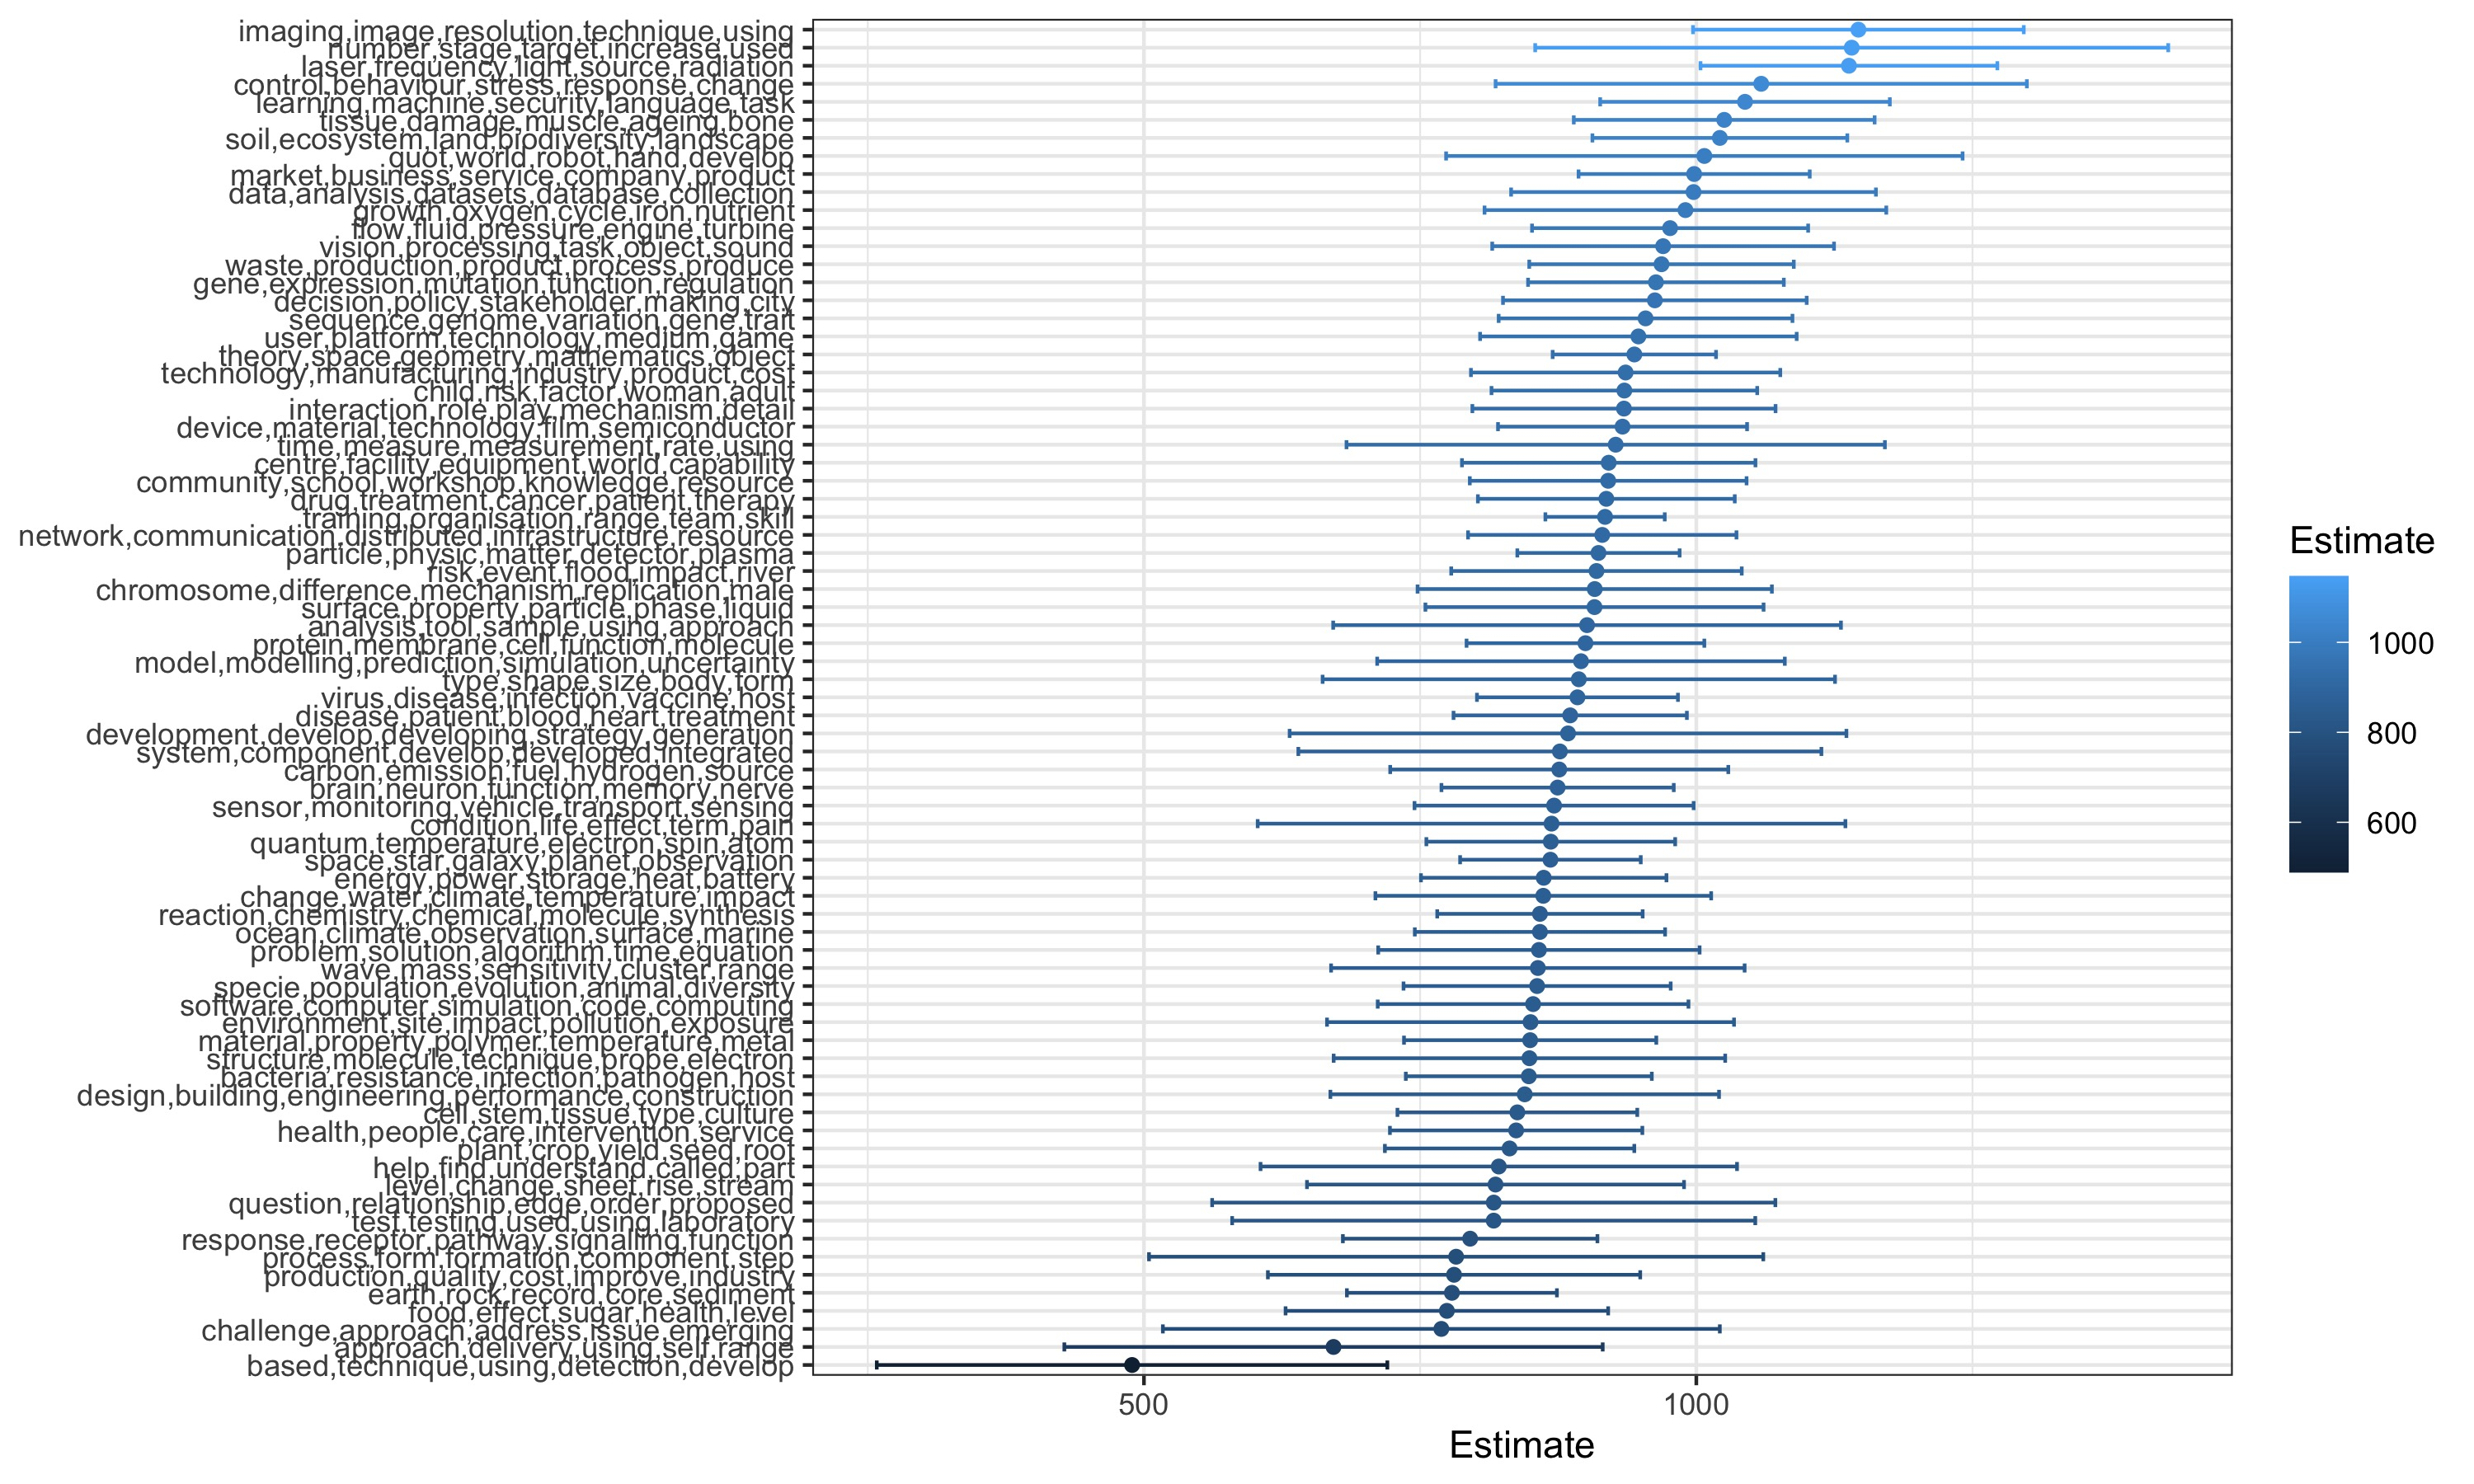
\includegraphics[width=18cm,height=13cm]{./figures/75-Duration}
    \caption{This figure shows the sLDA model labeled by project duration with 75 topics. The horizontal axis represents the coefficients within the sLDA model, which correspond to estimated values for various features. Meanwhile, the vertical axis signifies the different topics generated by the sLDA model. Each point in the figure represents a topic, and the numbers indicate their corresponding Estimate values. Error bars are included, and the upper and lower bounds are derived by adding or subtracting 1.96 times the standard error from the calculated estimate, which portray a confidence interval range of 95\%. }

\end{figure}

With the increase in the number of topics, the complexity of the model also grows, allowing it to better fit the data and capture more underlying structures and hidden patterns within the data. This enhanced complexity and flexibility enable the model to more accurately represent the text data and improve its ability to classify and categorize the documents effectively. As a result, the sLDA model demonstrates improved performance and becomes better equipped to address the complexities present in the dataset.\\\\

In the estimated coefficient plot of the sLDA model, if the utilized labels can effectively categorize the topics based on their ranking, then the sLDA model might exhibit improved performance. In the current scenario, there is significant overlap in the estimated values of project duration across different topics. This overlap could stem from the fact that the existing label information is insufficient to distinctly categorize the features related to project duration, leading to overlapping estimated values across various topics. This underscores the significance of labels in the sLDA model. The adequacy of label selection and utilisation can profoundly impact the outcomes and performance of the model. In summary, the sLDA model leverages labeled data to estimate the associations between topics and labels, providing a valuable tool for topic analysis and text classification.

\subsection{Topic Consistency by Human Judgements}
To enhance the credibility of our analysis in comparing LDA and sLDA, I
plan to incorporate human observations and judgments for high-frequency words related to each topic. This approach aims to provide a more dependable assessment. I will personally conduct an assessment of the top twenty most frequent words generated by each model. The selection of 225 topics is based on optimizing the LDA model's performance. I selected four similar topics from both the LDA and sLDA models to examine the topic words within each topic (as shown in Table 1 and Table 2). Within these topics, there are identical leading words.\\\\

Both LDA and sLDA utilize the Dirichlet distribution as a prior to generate the topic distribution of documents and the word distribution of topics, and employ methods such as Gibbs sampling for model training and inference, contributing to their inherent similarity in the topic generation process. Moreover, while sLDA introduces label information, there are cases where the impact of label information may not be substantial enough to significantly alter the way topics are generated. As a result, some topics in both models may exhibit similarities.\\\\

There is an example of viewing the topic words probability. In the topic 'machine learning' in both table 1 and 2, the majority of words are consistent, collectively focusing on aspects such as algorithm and intelligence, so it is not possible to determine which one is better. In the 'ecosystem' topic in LDA, the term 'service' holds a substantial probability, however, 'service' can link to many other topics. Despite this, due to its relatively high probability, the LDA model might inaccurately assign 'service' to the 'ecosystem' topic, potentially causing confusion in topic classification.\\\\

\begin{table}[H]
\centering
\begin{subtable}
\centering
\resizebox{\textwidth}{!}{%
\begin{tabular}{|p{0.15\textwidth}|c|p{0.8\textwidth}|}
\hline
\textbf{Topic} & \textbf{No.} & \textbf{Topic Words Generated by LDA Model} \\
\hline
Machine Learning & 64 & learning, machine, data, intelligence, algorithm, task, learn, classification, approach, technique, feature, improve, automated, reinforcement, time, domain, representation, supervised, trained, performance \\
\hline
Ecosystem & 39 & ecosystem, service, biodiversity, landscape, land, change, conservation, impact, habitat, benefit, scale, function, policy, restoration, community, reef, environment, food, knowledge, approach \\
\hline

\end{tabular}%
}
\caption{I choose some of topic words from the 225-topic LDA output, and summaries the topic name. The value of 'No.' corresponds to the position of the topic within the topic words matrix. The words are sorted in order of their probabilities of composing the topic.}

\centering
\resizebox{\textwidth}{!}{%
\begin{tabular}{|p{0.15\textwidth}|c|p{0.8\textwidth}|}
\hline
\textbf{Topic} & \textbf{No.} & \textbf{Topic Words Generated by sLDA Model} \\
\hline
Machine Learning & 44 & learning, machine, algorithm, intelligence, learn, inference, classification, representation, automated, statistic, task, carlo, monte, learned, reinforcement, supervised, setting, trained, segmentation, applied \\
\hline
Ecosystem & 221 & ecosystem, land, biodiversity, landscape, service, tree, forest, change, vegetation, climate, conservation, scale, habitat, poverty, disturbance, restoration, livelihood, functioning, degradation, agriculture \\
\hline



\end{tabular}%
}
\caption{This is the same as Table 1, but it represents the results from the 225-topic sLDA model.}
\end{subtable}
\end{table}


\begin{figure}[h]
    \centering
    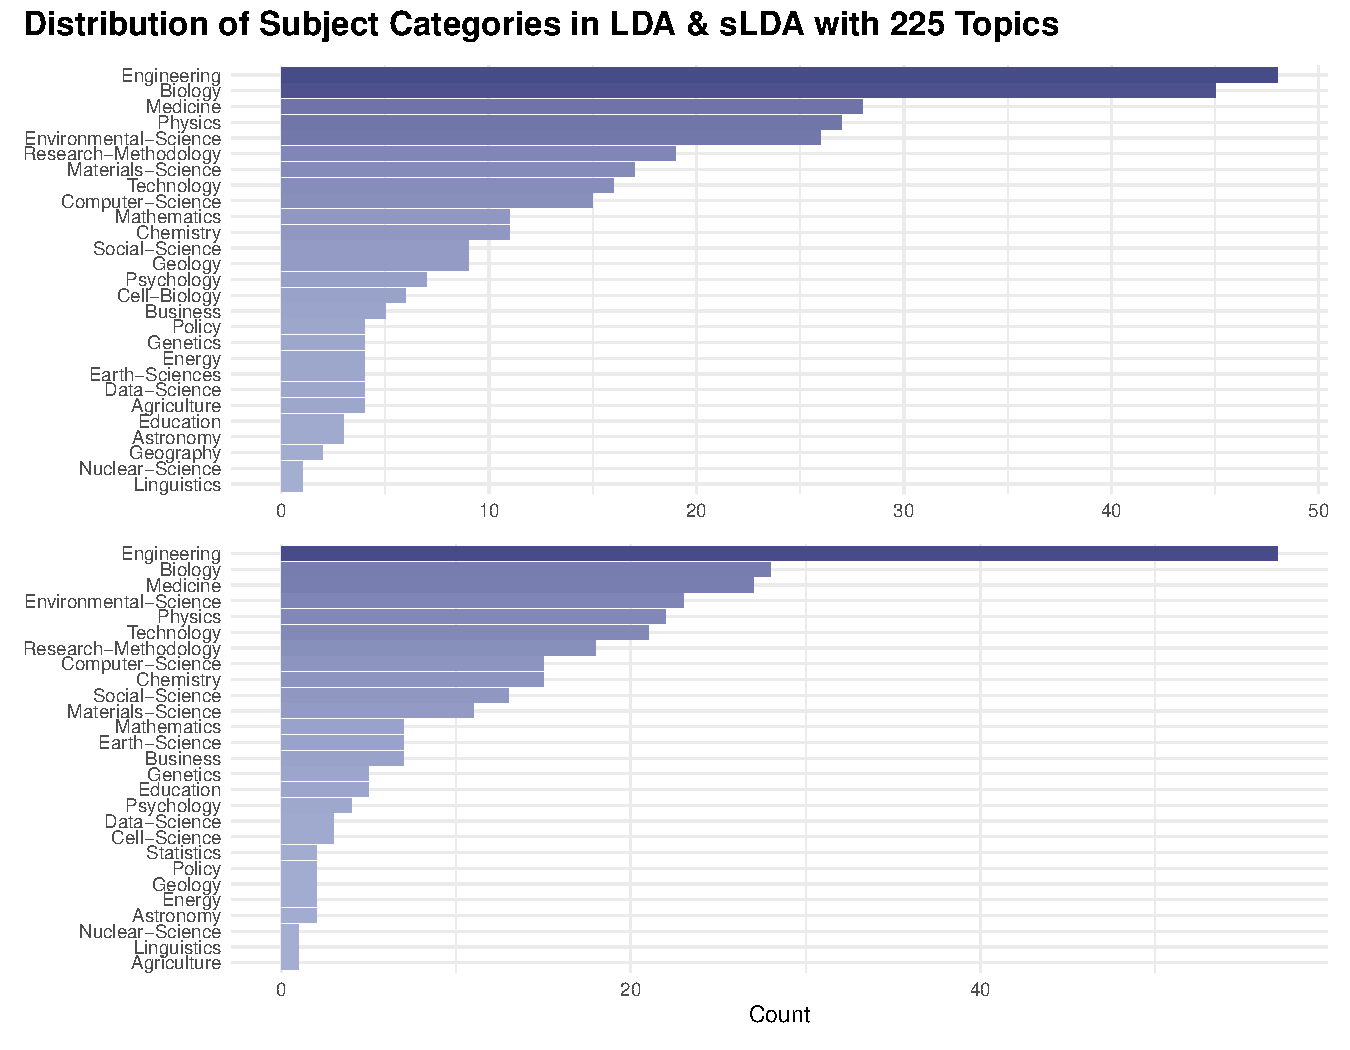
\includegraphics[width=15cm]{./figures/subject225}
    \caption{Subject Categories in 225-topic LDA and sLDA. The subject names have been summarized using a subject word frequency matrix. When examining topics resembling those depicted in Figure 1 (h, i), which primarily encompass terms such as "growth" and "impact" that lack explicit definitions and pose challenges for classification, I have categorized these topics under the "Research Methodology" and "Social Science" domains. }
\end{figure}

In Figure 5, I have conducted a subject classification using a topic words frequency matrix (for those subject name , I refer to 'chatgpt'). Given the vast scope of the scientific domain, which encompasses numerous subfields, I have undertaken the task of classifying these subjects into smaller, more specific branches.\\\\

It can be observed that the overall disciplinary categorization in both sLDA and LDA is similar within the 225 topics. This similarity might be attributed to the fact that both models utilize consistent priors. I found that in both LDA and sLDA model, also have some mean-less words. \\\\

Upon classification of the subject in both sLDA and LDA by myself, I observed that the topics in LDA are often a mixture of two distinct themes. This phenomenon leads to a higher count of subject categories in the LDA inference, most of which are related to biology. Specifically, the frequency of the term 'biology' is notably higher in LDA compared to sLDA. This suggests that in LDA, biological terms are repeatedly categorized across different topics. This multiple classification of biology-related vocabulary across various topics might indicate that the topic divisions in the LDA model are not as precise.\\\\

Based on the content of each topic, the majority of UKRI projects cover the field of science, followed by engineering, and then technology and mathematics. This distribution may be attributed to the relatively higher number of projects in the science domain within the UKRI portfolio. This observation potentially reflects the presence of extensive research, exploration, and innovative activities in the realm of science, thereby attracting a larger share of project funding and attention. While engineering, technology, and mathematics also have their share of projects, their representation might be comparatively lower, resulting in a reduced proportion within the overall project landscape. Such a distribution is likely influenced by a combination of factors including funding allocation, demand, research trends.

\newpage
\section{Discussion}

The ability of the LDA model to assist us in understanding relationships between topics, identifying commonalities, revealing latent themes, and addressing the complexity of word polysemy and semantic associations holds significant value for text analysis, topic mining, and information extraction.\\\\

The LDA model categorizes words with similar semantics or thematic associations together, thereby forming distinct characteristics for each topic. Additionally, this clustering of related vocabulary aids in understanding the relationships between different topics and identifying commonalities among them. This further reveals how the LDA model extracts hidden themes from extensive text data, and the generated topic-word frequency matrix allows us to perceive the importance of each word within a topic, thereby revealing underlying content within the topics. Lastly, LDA also highlight the complexity of word polysemy and semantic associations in various contexts, emphasizing that the same vocabulary might hold different meanings across different topics. In conclusion, these observations offer an effective approach for comprehending and analyzing the semantic and thematic relationships within textual data.\\\\

In the comparison of term coherence, concerning the term co-occurrence frequency metric within the co-occurrence matrix, LDA and sLDA exhibit similarities, but they may have different advantages under various topic scales. In terms of the metric reflecting the frequency differences between terms' co-occurrences, sLDA outperforms LDA, indicating that sLDA holds an advantage in capturing frequency disparities and semantic similarity among terms. sLDA also demonstrates greater efficacy in handling diversity, semantic relationships, and topic interactions. By incorporating label information, sLDA calculates larger term co-occurrence frequency differences, leading to higher values in assessing term coherence.\\\\

Similar topics and coherence matrices are generated in the sLDA model. This could be attributed to the relatively limited influence of label constraints on topic generation within the sLDA model, resulting in less distinct differences between topics associated with different labels. As a consequence, the coherence matrix exhibits similarities. If the labels used can clearly categorize the topics according to their ranks, this would lead to an improved performance of the sLDA model. Currently, there is significant topic overlap in the estimated values related to project duration. If more precise and distinct labels could guide the model, resulting in a clearer division of topics, it would help reduce topic overlap and enhance the model's performance and accuracy.\\\\

When calculating perplexity, the LDA model has a distinct optimal number of topics, while the sLDA model improves as the number of topics increases. This is because the sLDA model is designed to obtain more accurate estimates as the number of topics increases, which in turn exhibits better topic model classification capabilities. We can observe a significant difference in perplexity between the LDA and sLDA models, which could be attributed to the incorporation of label information in sLDA. The integrating of label information in sLDA through weighted parameters may control the influence of labels on the model, and the inclusion of estimated values could enhance predictive capabilities. Different weight settings might lead to varying degrees of label integration into the model. Consequently, sLDA exhibits superior predictive and categorization abilities when faced with new text data, thereby affecting perplexity. The LDA model is likely to be more complex, leading to high levels of confusion and resulting in a diminished ability to predict new text. The sLDA model is capable of acquiring more prior knowledge about the data structure, enhancing clustering effectiveness and promoting tighter grouping of texts within the same category. This enhancement further contributes to a reduction in perplexity. These findings hold significant implications for text analysis and topic modeling domains, offering potential directions and explanations for further research endeavors.\\\\

The estimation values of the sLDA model are obtained by optimizing the joint probability of text data and label information. During the training process, the model seeks the optimal parameter settings to maximize the likelihood of the data, and it determines the probability relationships between each topic and its associated labels. This assists in comprehending the structure and patterns within the text data, thereby leading to a better understanding of the content of the UKRI project. The sLDA model not only categorizes each topic but also generates estimation values to enhance the model's performance and predictive capabilities, facilitating label predictions for subsequent projects within the UKRI by leveraging the estimated values.\\\\

Through human judgment of the two models, it can be inferred that the LDA model may have some limitations in terms of topic classification accuracy, including potential topic mixing and some irrelevant words. On the other hand, the sLDA model, after incorporating label information, demonstrates an improved ability to address these issues and enhance its performance. While human judgment might not easily discern such differences, machine learning methods can offer more objective and accurate outcomes in performance evaluation. This underscores the significance of employing machine learning techniques for model performance assessment, facilitating a more comprehensive understanding of the models' performance in handling complex data.


\newpage
\section{Appendix}
\begin{figure}[h]
    \centering
    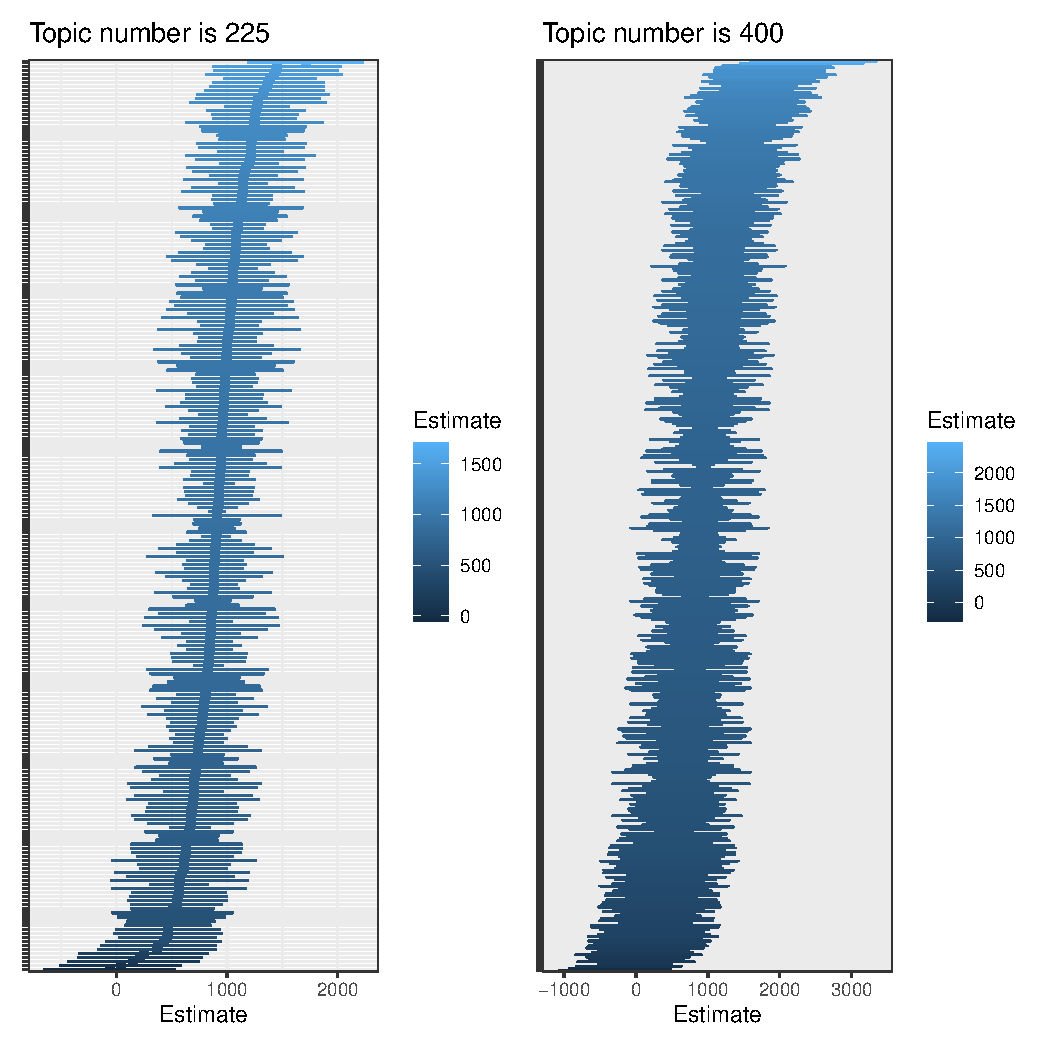
\includegraphics[width=15cm]{./figures/Durslda225&400}
    \caption{This figure shows the sLDA model labeled by funding body with 225, 400 topic }
    \label{fig:appendix A}
\end{figure}

\section{Data and Code Availability}
The data and code used in this study are available on [https://github.com/zitong27/Master-Project]. 

\newpage
\addcontentsline{toc}{section}{References}
\bibliography{coursework}
\end{document}